%%%%%%%%%%%%%%%%%%%%%%%%%%%%%%%%%%%%%%%%
%% MCM/ICM LaTeX Template %%
%% 2023 MCM/ICM           %%
%%%%%%%%%%%%%%%%%%%%%%%%%%%%%%%%%%%%%%%%
\documentclass[12pt]{article}
\usepackage{geometry}
\usepackage[ruled,vlined]{algorithm2e}

\geometry{left=1in,right=0.75in,top=1in,bottom=1in}

%%%%%%%%%%%%%%%%%%%%%%%%%%%%%%%%%%%%%%%%
% Replace ABCDEF in the next line with your chosen problem
% and replace 1111111 with your Team Control Number
\newcommand{\Problem}{E}
\newcommand{\Team}{2313746}
%%%%%%%%%%%%%%%%%%%%%%%%%%%%%%%%%%%%%%%%
\newcommand{\adots}{\mathinner{\mkern2mu%
        \raisebox{0.1em}{.}\mkern2mu\raisebox{0.4em}{.}%
        \mkern2mu\raisebox{0.7em}{.}\mkern1mu}}
%%%%%%%%%%%%%%%%%%%%%%%%%%%%%%%%%%%%%%%%

\usepackage{newtxtext}
\usepackage{amsmath,amssymb,amsthm}
\usepackage{newtxmath} % must come after amsXXX
\usepackage{setspace}
\usepackage{graphicx}
\usepackage{xcolor}
\usepackage{fancyhdr}
\usepackage{subfigure}
\lhead{Team \#\Team}
\rhead{}
\cfoot{}

\newtheorem{theorem}{Theorem}
\newtheorem{corollary}[theorem]{Corollary}
\newtheorem{lemma}[theorem]{Lemma}
\newtheorem{definition}{Definition}

%%%%%%%%%%%%%%%%%%%%%%%%%%%%%%%%
%================================
\usepackage{enumerate}%\item 需要
\usepackage{tabularx}% \table 
\usepackage{booktabs}% 	\toprule
\usepackage{float}%图片浮动
\usepackage{graphicx}
\usepackage{bm}% reference
\usepackage{indentfirst} 
\setlength{\parindent}{2em} %2em代表首行缩进两个字符
\usepackage{listings}%代码
\graphicspath{{Figure/}}
\usepackage{multirow}
\usepackage{caption}

%================================
\begin{document}
%\graphicspath{{.}}  % Place your graphic files in the same directory as your main document
%\DeclareGraphicsExtensions{.pdf, .jpg, .tif, .png}
\thispagestyle{empty}
\vspace*{-16ex}
\centerline{\begin{tabular}{*3{c}}
	\parbox[t]{0.3\linewidth}{\begin{center}\textbf{Problem Chosen}\\ \Large \textcolor{black}{\Problem}\end{center}}
	& \parbox[t]{0.3\linewidth}{\begin{center}\textbf{2025\\ MCM/ICM\\ Summary Sheet}\end{center}}
	& \parbox[t]{0.3\linewidth}{\begin{center}\textbf{Team Control Number}\\ \Large \textcolor{black}{\Team}\end{center}}	\\
	\hline
\end{tabular}}

%==========================================
\renewcommand{\abstractname}{Summary}
%=====================================
%%%%%%%%%%% Begin Summary %%%%%%%%%%%
% Enter your summary here replacing the (red) text
% Replace the text from here ...

\begin{center}
	\large\textbf{  {The Strategies for Seeing the Milky Way Again 
	}}
	\end{center}
\begin{abstract}
%%%%%%%%%%   摘要开始 摘要开始 摘要开始 摘要开始                  %%%%%%
%开头段

\begin{center}
    \textit{Only in the darkness can you see the stars  ——Martin Luther King JR.}
\end{center}
\\

How long has it been since you've seen the Milky Way? According to the latest research, about $80\%$ of people worldwide live under light pollution that prevents them from seeing the Milky Way, and $99\%$ of people in the United States and Europe live under light-polluted skies. This surprised and saddened us. To better measure the risk level of light pollution\textbf{(LPR)}, we established a light pollution risk assessment system and developed three intervention strategies to mitigate the risk of light pollution.

First, we integrated the mechanism analysis and comprehensive evaluation modelto establish the \textbf{Comprehensive LPR Evaluation Model}. Since the environment is different in different communities and therefore the light pollution sources are different and cause different impacts, the light pollution risk level should take into account the level of light pollution and the possible impact of light pollution on the local area. We define them as the degree of light pollution \textbf{(LPD)}and the level of light pollution impact\textbf{(LPI)}, respectively. 

In order to determine the exact value of LPD and LPI, We use the mechanism analysis method to calculate the LPD by using the data of night sky brightness, altitude, climate, etc. We use the \textbf{entropy weighting method(EWM)}  to determine the weight of light pollution on human health, ecological environment, resource waste, traffic safety and use the \textbf{Topsis method}  to calculate the LPI, and finally we get the LPR by combining the two by \textbf{Formula (1)}.

Then, we selected four different types of communities to apply our model, they are:protected land location: Yellowstone National Park; rural community: Asheville; suburban community: Westminster and urban community: Manhattan , with LPA of \textbf{0.036, 0.235, 0.152, }and \textbf{0.757}. For more results see \textbf{Figure 8} ,and \textbf{Table 5}, unexpectedly the LPR is lower in our selected suburban than in rural areas, which we believe is mainly due to the different levels of development in the countries where they are located.

Based on the previously constructed indicators affecting the level of light pollution risk, three intervention strategies were developed to mitigate light pollution risk: \textbf{Strategy 1}: reduce lighting hours, \textbf{Strategy 2}: replace lighting fixtures, and \textbf{Strategy 3} : optimize urban traffic e-light devices. Their main effect is to reduce the level of light pollution and the waste of resources, while strategy 2 can also reduce the impact on human health and the ecological environment. For a more detailed discussion of these strategies see \textbf{Section 7}.

In addition, we estimated the possible impacts of our intervention strategies in Manhattan and Asheville. For this purpose we divided the lighting levels of Manhattan and Asheville into zones according to their \textbf{lighting needs}, and then used our strategies to intervene. We investigated the impact of each policy alone and all policies together. In both areas, the ranking of the policies from best to worst was always Strategy 2 $>$ Strategy 1 $>$ Strategy 3. For both areas, our intervention strategy had a more significant impact on Manhattan, in fact, when we used Strategy 2, the LPR in Manhattan decreased from \textbf{0.757} to \textbf{0.655}, a reduction of \textbf{19.20\%}.For Asheville, these values are  \textbf{0.235} ,\textbf{0.206} ,\textbf{18.70\%.} For more results, please see\textbf{Figure 11-14}  and \textbf{Table 6}.

Finally, We performed a \textbf{sensitivity analysis} of the model. For the parameters $b$ and $C$ , when changing them by 10\%, the results changed very little, indicating that our model is stable for these two parameters.

\textbf{Keywords}: Light Pollution, Mechanism analysis ,EWM ,Topsis,Sensitivity Analysis
\end{abstract}
% to here
%%%%%%%%%%%      摘要结束 摘要结束 摘要结束 摘要结束              %%%%%%%%%%%

%%%%%%%%%%%%%%%%%%%%%%%%%%%%%%
\clearpage
\pagestyle{fancy}
% Uncomment the next line to generate a Table of Contents
\begin{spacing}{1.3}
\small\tableofcontents
\end{spacing}
\rhead{Page 2 of 25}
\newpage
\setcounter{page}{3}
\rhead{Page \thepage\ of 25}
%%%%%%%%%%%%%%%%%%%%%%%%%%%%%%
\section{Introduction}
\subsection{Problem Background}
Light pollution is one of the fastest growing and most pervasive of environmental pollution$^{[1]}$. It has become a significant issue in modern times, with the increased use of artificial light in urban areas and other locations around the world. It is caused by the excessive or inappropriate use of lighting, which can have negative effects on the environment, human health, and safety. Light pollution can cause a range of phenomena, including light trespass, over-illumination, and light clutter, all of which can lead to the alteration of our view of the night sky. Additionally, light pollution can impact plant growth and wildlife migration patterns, as well as disrupt human circadian rhythms, leading to sleep and health issues. 

 \begin{figure}[h]
	%图片浮动 
	%h(here)-代码所在的上下文位置
	%t(top)-代码所在页面或之后页面的顶部
	%b(bottom)-代码所在的页面或之后页面的底部
	%p(page)-独立一页的浮动页面
	
	\centering
	%居中
	
\includegraphics[width=0.7\textwidth]{/The night sky with and without light pollution.jpg}
	%标题 \label命令设置标签
	\caption{The night sky with and without light pollution}
	\label{The night sky with and without light pollution}
\end{figure}


To mitigate these negative effects, community officials and local groups may implement intervention strategies. However, there are also positive effects of artificial light, such as increased safety and productivity, which can impact different locations in different ways. Therefore, addressing light pollution requires a tailored approach that takes into account factors such as development level, population, biodiversity, geography, and climate, to assess the potential impacts of any intervention strategies.

%\begin{enumerate}[\quad\bf]
%Light pollution is one of the fastest growing and most pervasive of environmental pollution [1]. It has become a significant issue in modern times, with the increased use of artificial light in urban areas and other locations around the world. It is caused by the excessive or inappropriate use of lighting, which can have negative effects on the environment, human health, and safety. Light pollution can cause a range of phenomena, including light trespass, over-illumination, and light clutter, all of which can lead to the alteration of our view of the night sky. Additionally, light pollution can impact plant growth and wildlife migration patterns, as well as disrupt human circadian rhythms, leading to sleep and health issues. 
%To mitigate these negative effects, community officials and local groups may implement intervention strategies. However, there are also positive effects of artificial light, such as increased safety and productivity, which can impact different locations in different ways. Therefore, addressing light pollution requires a tailored approach that takes into account factors such as development level, population, biodiversity, geography, and climate, to assess the potential impacts of any intervention strategies.


%\end{enumerate}
\subsection{Restatement of the Problem}
Considering the background information and restricted conditions identified in the problem statement, we need to solve the following problems:
\begin{itemize}
	\item  Create a metric that can be widely used to assess the level of light pollution risk in any given location. Then, utilize this metric to evaluate and analyze the light pollution risk in four types of locations: A protected land location, a rural community, a suburban community, and an urban community. Finally, interpret the results of the metric.
	\item  Derive 3 intervention measures by establishing different intervention strategy functions, and discuss the specific actions and potential impacts of each action.
	\item  Select two locations and employ the metric to determine the most effective intervention strategy for each of them. Analyze the impact of the selected intervention strategy on the risk level of the respective location.
    \item  Produce a one-page promotional flyer that promotes the selected intervention strategy as the optimal solution for addressing light pollution in one of the identified locations.
\end{itemize}
\subsection{Literature Review}
A large number of researchers have made great contributions to this question.

Light pollution is a growing concern in our modern world because it wastes energy, endangers our health and disrupts the natural rhythms of the Earth.$^{[11]}$ From reading the literature, we know that light pollution can be broadly classified into two types: natural pollution and man-made pollution. Among them, the most important and common form of light pollution comes from artificial lighting sources.

Artificial light pollution sources can be roughly divided into indoor lighting and outdoor lighting. Indoor lighting includes devices such as TVs, computer screens and smartphones, which emit blue light that interferes with our sleep patterns and circadian rhythms.

Outdoor lighting is probably the most significant contributor to light pollution in urban, suburban and rural areas. Many of these lights use outdated and wasteful fixtures that emit excessive glare and produce unwanted sky glow.$^{[6]}$

Sources of light pollution are influenced by a variety of factors, including geographic location, time of day and season, weather conditions, type and intensity of light sources, local regulations and policies, public awareness and education, altitude, cloud thickness, average building height, and duration of public lighting. 

One of the most obvious effects of light pollution is that the night sky becomes blurred, which can make it difficult to see stars and other celestial bodies$^{[7]}$, which hinders scientific research and education. In addition, light pollution not only interferes with the natural rhythms of plants and animals$^{[2]}$, but can also have adverse effects on our health, such as disrupting our sleep patterns and circadian rhythms, leading to a variety of health problems such as insomnia, obesity and depression. 

In conclusion, light pollution is a growing problem, and understanding its sources and effects, as well as the factors that influence it, is critical to developing effective solutions to reduce its impact. By promoting the responsible and efficient use of artificial lighting, we can help preserve the natural beauty of the night sky, protect our health and well-being, and ensure a more sustainable and harmonious relationship between humans and the natural environment.
\subsection{Our work}
This problem requires us to construct methods to measure the level of light pollution risk and to specify relevant strategies to mitigate the effects of light pollution,Our work mainly includes the following:



\begin{enumerate}[\bf 1).]
        \setlength{\itemindent}{2em} 
	\item Based on the data about light pollution, a comprehensive evaluation model of LPR is established.
	\item Developed intervention strategies to mitigate the effects of light pollution.
	\item Predicted the impact of our intervention strategy.

\end{enumerate}

In order to avoid complicated description, intuitively reflect our work process, the flow 
chart is shown in Figure \ref{our work}.

\begin{figure}[h]
%图片浮动 
%h(here)-代码所在的上下文位置
%t(top)-代码所在页面或之后页面的顶部
%b(bottom)-代码所在的页面或之后页面的底部
%p(page)-独立一页的浮动页面

        \centering
%居中
        
\includegraphics[width=1\textwidth]{/our work.png}
%标题 \label命令设置标签
        \caption{Our Work}
        \label{our work}
    \end{figure}

\section{Assumptions and Justifications}

To simplify the problem, we make the following basic assumptions, each of which 
is properly justified.
\begin{itemize}
    \item \textbf{Assumption:}We assume that the data obtained are accurate and reliable.

    \textbf{Justification:}We get data from trusted websites and papers.
    \item \textbf{Assumption:}differences in light pollution sources, climate, and biodiversity within the community are negligible.

    \textbf{Justification:}Although there are differences in conditions within communities, the differences within communities are small compared to the differences between communities and are therefore negligible and considered the same.
    \item \textbf{Assumption:}The level of light pollution in the community is stable over a short period of time and is not affected by unexpected events.

    \textbf{Justification:}According to the data, the severity of light pollution varies less than 3\% every year, and the probability of unexpected events, such as power outages due to disasters, is low, so we can ignore these problems and consider the light pollution level to be stable in a short period of time.
    \item\textbf{Assumption:}
The light pollution levels of the characteristic responses calculated by the different methods in the data are the same.

    \textbf{Justification:}
    The evaluation methods used in our dataset are scientifically rigorous and have been used in institutional research and governmental decision making, so although different evaluation methods are used in different regions, it can be assumed that the pollution levels are the same in the same region using different methods.
\end{itemize}

%假设1:We assume that the data obtained are accurate and reliable

%解释:We get data from trusted websites and papers
%假设2 ：社区内部的光污染源，气候，生物多样性等条件的差异可以忽略不计.

%解释：虽然社区内部的各种条件有所差异，但是与不同社区的之间的差异相比时内部的差异是微小的，因此可以忽略不计，认为是相同的.

%假设3：社区的光污染程度在短时间内是稳定的,不会受到突发事件影响。

%解释：根据数据显示光污染的严重程度每年提高百分之3，同时发生突发事件,例如因灾难导致停电等事情发生概率低,因此可以忽略这些问题,认为光污染程度在短时间内是稳定的.

%假设4：数据中不同的方法计算出的特征反应的光污染水平是相同的

%解释：我们使用的数据集中采用的评价方法都是经过严密的科学论证下计算出的结果并且已经在机构的研究，政府的决策中被使用，因此虽然不同地区的采用评价方法不同，但是可以认为在同一地区使用不同方法得出的污染水平是相同的。


Additional assumptions are made to simplify analysis for individual sections. These as-
sumptions will be discussed at the appropriate locations.

%%%                     符号说明             %%%%%%%%%%
\section{Notations}

The symbols  in  \textbf{Table \ref{Notations}} are frequently used in the model construction. Others will be introduced when they are used.

\begin{table}[H]
	\begin{center}
		\caption{Notations}
		\begin{tabular}{cccc}
			\toprule
			\multicolumn{1}{m{1cm}}{\centering Symbol}
			&\multicolumn{1}{m{10cm}}{\centering Definition}
                &\multicolumn{1}{m{2cm}}{\centering Unit}\\
			\midrule
   $L_{\text{sqm}}$&The Brightness Of the Night Sky &$\text{M}/\text{arcsec}^2$\\
			$\Phi$&Luminous Flux&lm\\
			$Ev$&Illuminance&lx\\
			$T$&Average Lighting Hours&h\\
			$H$&Altitude&m\\
            $\text{HL}$&Effect of Altitude on Light Pollution&\textbackslash\\
                $F_c$&Fraction of Cloud Cover&\textbackslash\\
                $\text{LPD}$&The Degree of Light Pollution&\textbackslash\\
                $\text{LPI}$&The Impact of Light Pollution&\textbackslash\\
                $\text{BI}$&Biodiversity Intactness&\textbackslash\\
                $\rho_N$&Population Density&People /k$\text{m}^2$\\
                $\text{PL}$&Light pollution impact levels on human heath risks&\textbackslash\\
                $\text{BL}$&Light pollution impact level on ecological risk&\textbackslash\\
                $\text{TL}$&The Impact of light pollution on traffic safety risk&\textbackslash\\
                $\text{EL}$&The Level of Light Pollution Impact on Resource Waste&\textbackslash\\
                $\text{LPR}$&The Level of Light Pollution Risk &\textbackslash\\
			\bottomrule
		\end{tabular}\label{Notations}
	\end{center}
\end{table}

 \section{Data Collection}
In order to build the model, we need to collect some data about geography, environment, people, light pollution, etc.The data sources are shown in Table \ref{Data Sources}.
\begin{table}[H]
 \begin{center}
  \caption{Data Sources}
  \label{Data Sources}
  \begin{tabular}{cc}
   \toprule
   \multicolumn{1}{m{3cm}}{\centering Database Names}
   &\multicolumn{1}{m{8cm}}{\centering Database Websites}\\
   \midrule
   Light pollution map&https://www.lightpollutionmap.info/\\
   ERA5&https://cds.climate.copernicus.eu/\\
   Biodiversity   Intactness&https://map.unbiodiversitylab.org/\\
   Altitude&https://search.earthdata.nasa.gov/search\\
   Google Scholar&https://scholar.google.com/\\
   \bottomrule
  \end{tabular}\label{Ntt}
 \end{center}
\end{table}

\section{Comprehensive LPR Evaluation Model}
In order to measure the effect of light pollution, we constructed the \textbf{Comprehensive LPR Evaluation Model}. In order to construct this model, we need to know what the risk level of light pollution is related to. First, the level of light pollution (LPD) is different in different regions due to environmental and economic differences, and the impact of light pollution (LPI) is also different (e.g., light pollution in cities mainly affects human health, and in protected areas mainly affects the ecological environment). Therefore, the risk level should be considered together with both.

Léa Mariton et al. have pointed out that even low levels of light pollution can have an impact on biological health$^{[2]}$. It is also predictable that the higher the pollution level, the greater the impact is, so we use
$\text{LPR}=\frac{\text{LPI}\cdot\ln(\text{LPD}+C)}{\ln(C+1)}$
to calculate LPR. Here C is a constant that affects the weight of two indicators on the final result, and according to our experiments, it is found that C is better when it is taken as 2.
%取C等于2
Therefore, to calculate the risk level, the actual formula is

\begin{equation}
\text{LPR}=\frac{\text{LPI}\cdot\ln(\text{LPD}+2)}{\ln3},
\end{equation}


where LPD and LPI are unitary assessment indicators, and their values are in the range of [0,1], the larger the value, the more serious the pollution (impact). The detailed construction process will be explained later. In order to unitize, we divide by ln3 here, so that the LPR calculated by this formula is also in the range of [0,1].
%Léa Mariton, Christian Kerbiriou, Yves Bas, Brigitte Zanda, Isabelle Le Viol,Even low light pollution levels affect the spatial distribution and timing of activity of a “light tolerant” bat species,Environmental Pollution,Volume 305,2022,119267,ISSN 0269-7491,https://doi.org/10.1016/j.envpol.2022.119267.(https://www.sciencedirect.com/science/article/pii/S026974912200481X)

We use ln(LPD+1) in order to make the term constant, ensuring its monotonicity while growing more slowly when the LPD is larger (in reality it does not have a greater impact when the threshold value is exceeded). At the same time, in order to ensure that the LPR remains in the range of [0,1].
This formula reflects the characteristics of light pollution risk, i.e. the higher the level of pollution the greater the impact, and the local environmental and social conditions have a greater impact on the risk.

Next, we need to calculate the light pollution level LPD and the light pollution impact LPI specifically.
\subsection{The Degree of Light Pollution(LPD)}
There are many ways to evaluate the level of light pollution. We can count the number of lights in a city, the brightness of lighting and other information to calculate it. But such information is too tedious to obtain, or even difficult to obtain. In the following, we will use four types of data that are easier to obtain and more accurate to judge the degree of light pollution.

\begin{itemize}
\item\textbf{Sky Brightness}

 From the Light Pollution Map, we can get some data on the brightness of the night sky collected by scientists and private enthusiasts. The data here are usually collected using the SQM instrument, which measures the brightness of the night sky to reflect the level of light pollution. The lower the value, the higher the level of pollution. For the SQM series instruments, the measurement range is 16-22 mag/$\text{arcsec}^2$,
For the sky brightness, the dark sky should be darker than 24 mag/$\text{arcsec}^2$, and under natural conditions, the average sky brightness should be 21.9 mag/$\text{arcsec}^2$. When the sky brightness reaches 10.5 mag/$\text{arcsec}^2$ or even brighter, all the components that help to observe the night sky will disappear.
\begin{figure}[h]
%图片浮动 
%h(here)-代码所在的上下文位置
%t(top)-代码所在页面或之后页面的顶部
%b(bottom)-代码所在的页面或之后页面的底部
%p(page)-独立一页的浮动页面

        \centering
%居中
        
\includegraphics[width=1\textwidth]{/Sky Brightness in V Magnitudes per square arc second - Weighting Factor Graph.png}
%标题 \label命令设置标签
        \caption{Sky Brightness in V Magnitudes per square arc second - Weighting Factor Graph$^{[6]}$}
        \label{Sky Brightness in V Magnitudes per square arc second - Weighting Factor Graph}
    \end{figure}
    %Green, R.F., Luginbuhl, C.B., Wainscoat, R.J. et al. The growing threat of light pollution to ground-based observatories. Astron Astrophys Rev 30, 1 (2022). https://doi.org/10.1007/s00159-021-00138-3

    
    From Figure \ref{Sky Brightness in V Magnitudes per square arc second - Weighting Factor Graph} and other information, we know that the sky quality varies considerably around the value of 20.5, and the pollution level changes less when it is too strong and too dark, so we consider using the Sigmod function to normalize the SQM value. Since the larger the SQM value represents the better quality, and we hope that the larger the value of the final indicator represents the worse quality. Therefore we determine the Sigmod function as
    \begin{equation}
L_{\text{sig}}=\frac{1}{1+e^{2(L_{\text{sqm}}-20.5)}}
\end{equation}
It can be seen that the value of SQM is very small (less than 0.05) when it is greater than 22, and when its SQM value is less than 19, its value is greater than 0.95. This indicates that the pollution level is serious. This is consistent with the actual situation.
\item\textbf{Duration of light}

Although the night sky brightness can be a good response to the degree of light pollution, but still not perfect, for example, when measuring the night sky brightness we often take the maximum value, and different areas of public lighting hours vary. It is easy to judge that the longer the public (average) lighting time, the more serious the pollution level. Here we still need to standardize the public lighting hours, considering that in most areas the lights are not on all night, so we use the min-max method to standardize, considering that there are still areas without lighting equipment, so here we take the minimum value of light hours to be zero, so the effect of light hours is
\begin{equation}L_T=\frac{T}{T_{max}}.\end{equation}
\item\textbf{Altitude}

Besides, altitude is a vital indicator to describe the degree of light pollution. It is easy to think that the higher the altitude, the greater the light exposure, which leads to a greater impact of light pollution, as you can see in Figure \ref{Effect of Altitude on the Degree of Light Pollution} below. 

    \begin{figure}[h]
%图片浮动 
%h(here)-代码所在的上下文位置
%t(top)-代码所在页面或之后页面的顶部
%b(bottom)-代码所在的页面或之后页面的底部
%p(page)-独立一页的浮动页面

        \centering
%居中
        
\includegraphics[width=0.9\textwidth]{/Effect of Altitude on the Degree of Light Pollution.png}
%标题 \label命令设置标签
        \caption{Effect of Altitude on the Degree of Light Pollution}
        \label{Effect of Altitude on the Degree of Light Pollution}
    \end{figure}
    
Here we ignore the effect of light reflection on the ground. We assume that the earth is a sphere with a radius of 6371km, and assume that the lighting fixtures used in different areas are the same. The altitude is $h_1$ and the average building height is $h_2$. And note that $h=h_1+h_2$. We know that the luminous flux is the luminosity multiplied by the area
$\Phi=Ev \times S$. 
Since the luminaires used are the same, we only need to calculate the illuminated area. According to Fighre\ref{Effect of Altitude on the Degree of Light Pollution} above and the simple knowledge of trigonometric functions we can know that 

\begin{gather}
    \cos\theta=\frac{L^2+(R+h)^2-R^2}{2L(R+h)}\\
    \frac{R}{\sin\theta}=\frac{L}{\sin\theta'}
\end{gather}

With the help of calculus, we can calculate the area of the sphere crown as
\begin{equation}\iint dS=2\pi R^2(1-\cos\theta')\end{equation}
Since $R$ is much larger than $h$, we can know that the area is proportional to $h^2$ according to the calculation result, thus defining 
\begin{equation}H_i=\frac{h^2}{h_{\max}^2}\end{equation}

The altitude not only affects the radiation range of light, but also the closer it is to the sky, the more light will reach the sky, which will lead to more serious light pollution, and the light reflected from the clouds to the ground will also increase, seen in Figure \ref{night}.
 \begin{figure}[htp]
%图片浮动 
%h(here)-代码所在的上下文位置
%t(top)-代码所在页面或之后页面的顶部
%b(bottom)-代码所在的页面或之后页面的底部
%p(page)-独立一页的浮动页面
\centering
    \subfigure[111]{
        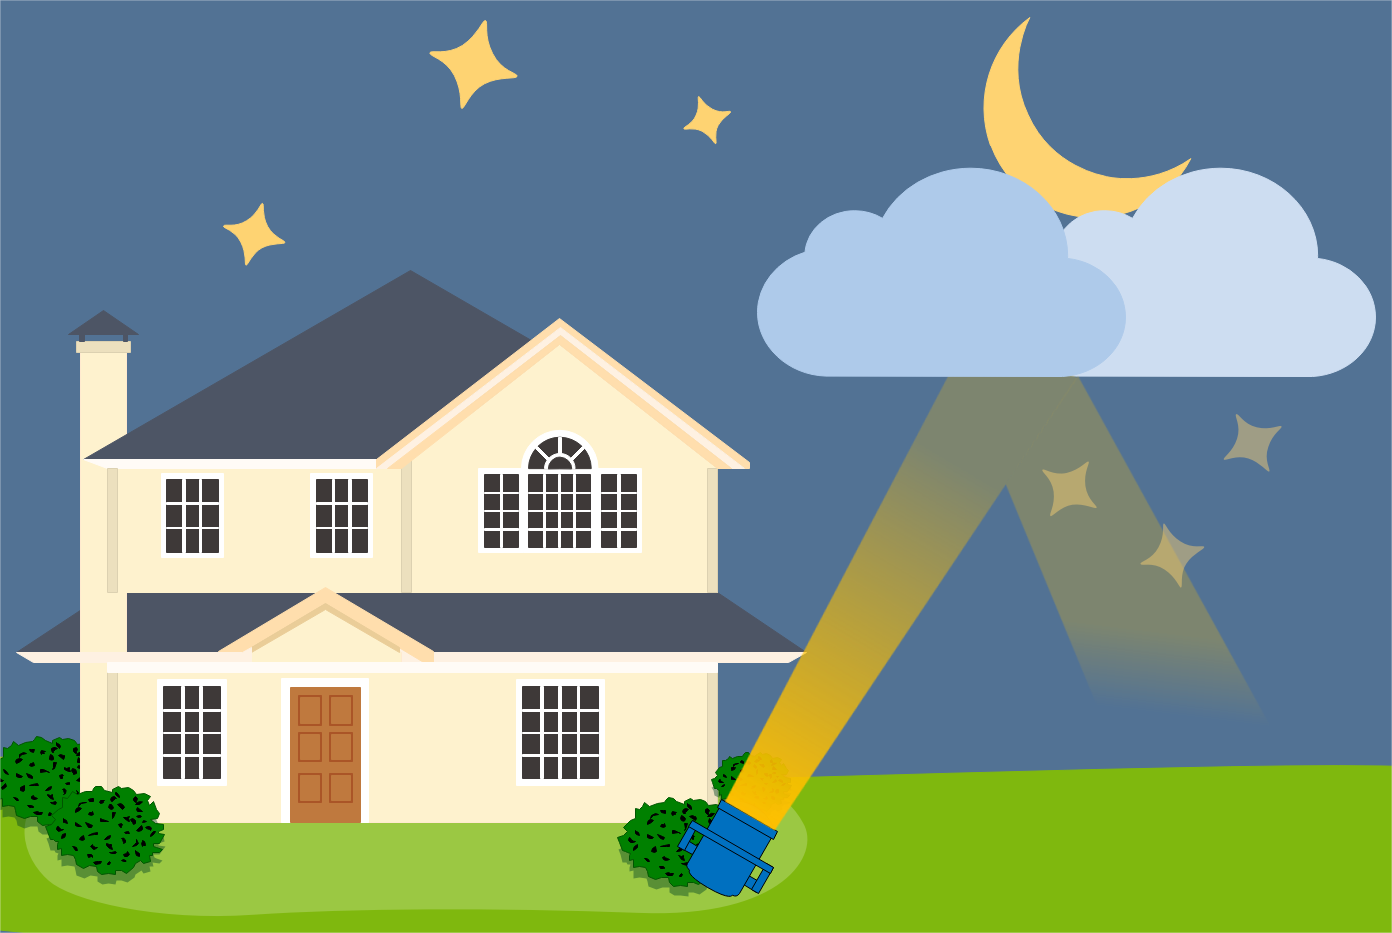
\includegraphics[width=0.2\textwidth]{Figure/night.png}
    }
    \hspace{0.01\textwidth} % Horizontal space between images
    \subfigure[222]{
        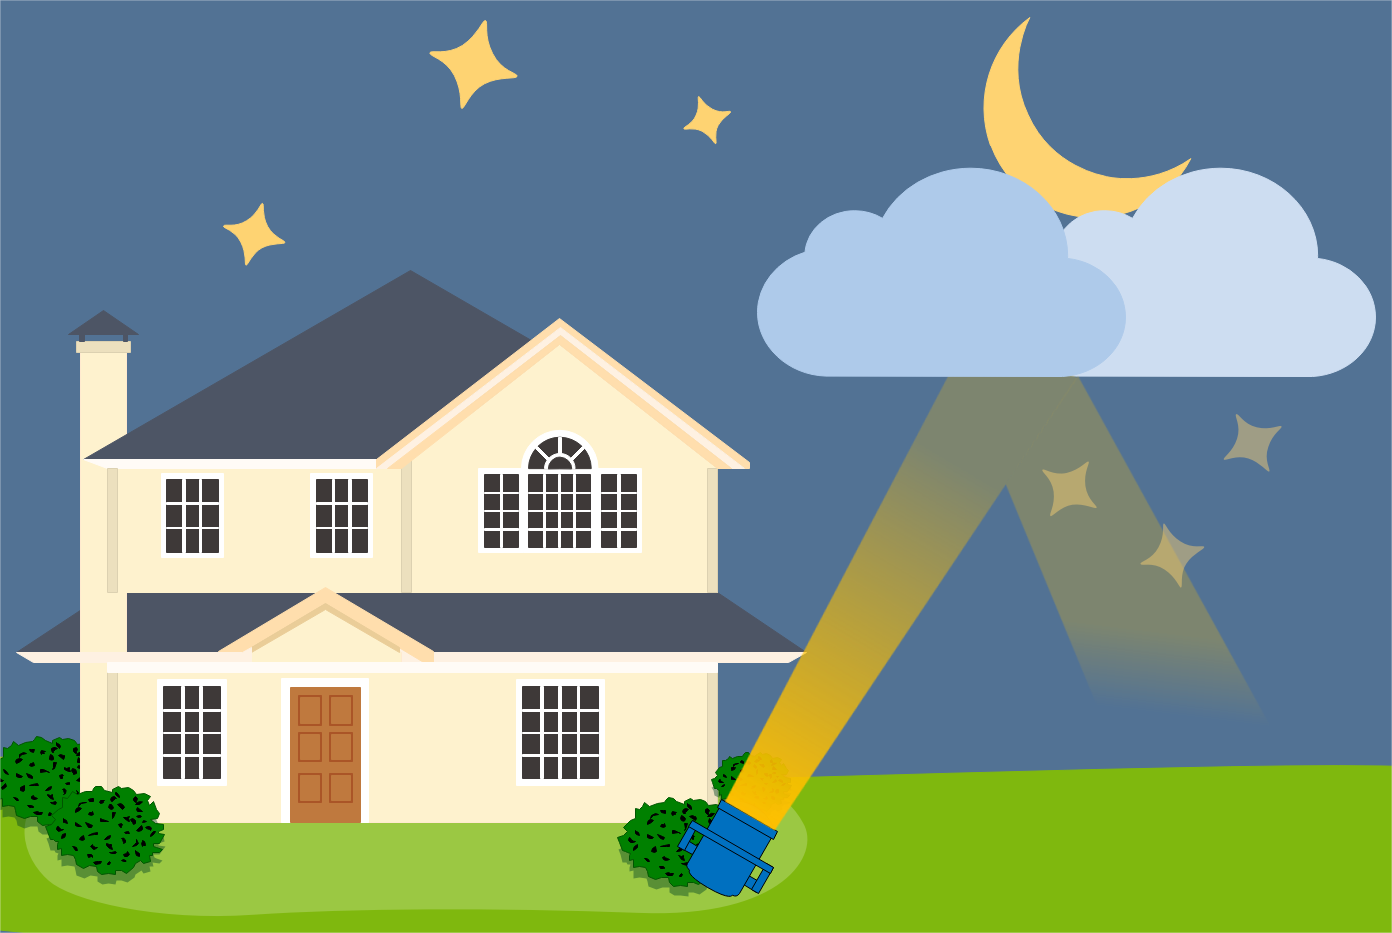
\includegraphics[width=0.2\textwidth]{Figure/night.png}
    }
    \hspace{0.01\textwidth} % Horizontal space between images
    \subfigure[333]{
        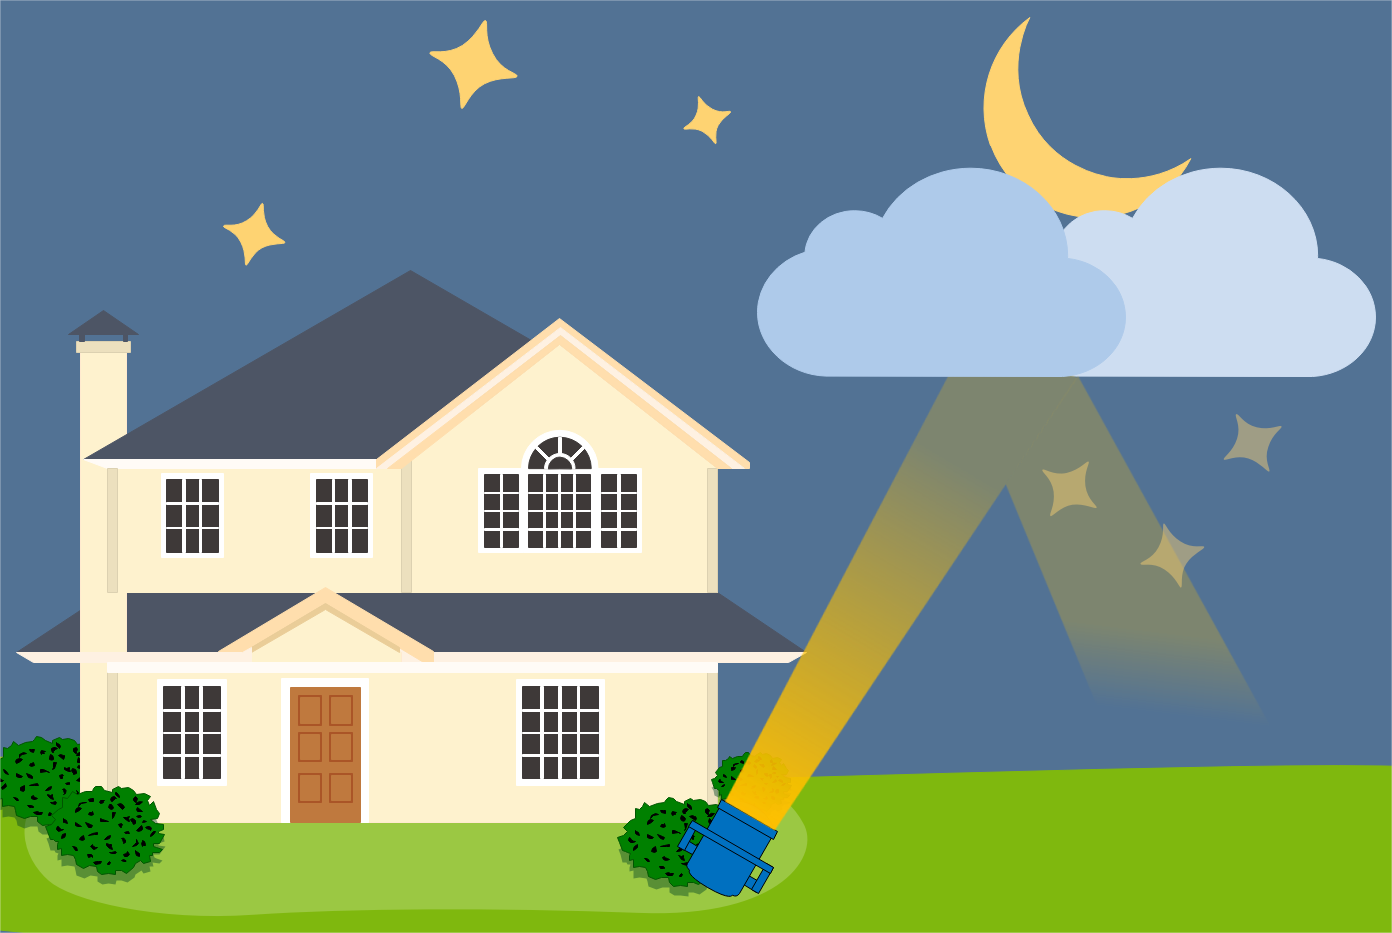
\includegraphics[width=0.2\textwidth]{Figure/night.png}
    }
    \caption{1111}
    \end{figure}
However, since the clouds are far from the ground, we do not consider the effect of altitude on this aspect.
\item\textbf{Climate}

Atmospheric conditions, which play an important role in light pollution, are evaluated using the cloud coverage ratio $F_c$ from the ERA5 database, defined as This parameter is the proportion of a grid box covered by cloud (liquid or ice) and varies This parameter is available on multiple levels through the atmosphere. Since it is already unitized data, we do not need to deal with it anymore.


\end{itemize}In summary, we define the degree of light pollution

\begin{equation}\text{LPD}=\frac{1}{1.2\times 1.5}L_{\text{sig}}(1+0.2L_T)(1+0.1H_i+0.05F_c).\end{equation}\textbf{ The Light Pollution Level is the main influence factor}, besides the light time, altitude and cloud cover ratio also have an influence, but the influence is small.
\subsection{The Impact of Light Pollution(LPI)}
Before understanding the light pollution impact degree LPI, We need to discuss the advantages and disadvantages of artificial light first.

\begin{itemize}

    \item \textbf{Artificial light affects human health.}

Artificial light can have various negative impacts on human health. One of the most significant effects is the disruption of the human circadian rhythm, which can lead to insomnia and poor sleep quality. This is due to the suppression of melatonin secretion, which is a hormone that regulates sleep-wake cycles. Prolonged exposure to strong artificial light sources can also cause eye health issues such as eye fatigue, dryness, and vision loss.  Artificial light can also cause psychological health issues such as depression and anxiety. Artificial light can potentially affect children's sleep, vision, and brain development due to their delicate eyes and circadian rhythms.


\item\textbf{Artificial light causes traffic hazards.}

Artificial light can negatively impact traffic in several ways. First, overly strong or glaring artificial light sources can cause drivers to feel dizzy and experience visual fatigue, reducing driving safety. Additionally, excessive use of artificial light sources may create glare or flashes, causing the driver's vision to become blurred or increasing the blind spots, thus increasing the risk of traffic accidents. Strong artificial light can also impair the visibility of pedestrians and cyclists, especially at night, increasing their risk on the road.


\item\textbf{Artificial light affects the ecological environment.}$^{[3][4]}$

Artificial light can have significant negative impacts on the ecological environment, as well as human health. The impact on the ecological environment includes disrupting the behavior and biological rhythms of animals and plants, such as the migration and habitat behavior of birds and the growth and reproduction of insects. Additionally, extensive use of artificial light sources consumes large amounts of energy and resources 
%like coal and gas, increasing energy emissions such as carbon dioxide and sulfur dioxide, and causing light pollution that damages astronomical observation and biological ecosystems. 
Furthermore, artificial light sources can affect human circadian rhythms and sleep quality, increasing the risk of diseases such as cardiovascular disease, diabetes, and obesity. 

\item\textbf{Artificial light causes waste of resources.}

In addition to the negative impacts on human health and the environment, the use of artificial light can also result in the wastage of resources, mainly in the following aspects: extensive energy consumption, leading to the generation of greenhouse gases and further exacerbating climate change.
%lighting waste due to continuous lighting modes, which waste energy and funds; and resource waste from the production and processing of artificial light sources, which requires a significant amount of limited resources and energy.
%%%%%IDA estimates that least 30 percent of all outdoor lighting in the U.S. alone is wasted, mostly by lights that aren’t shielded. That adds up to $3.3 billion and the release of 21 million tons of carbon dioxide per year! To offset all that carbon dioxide, we’d have to plant 875 million trees annually.
\end{itemize}

But artificial light isn't all about drawbacks. Artificial light improved productivity by extending the hours of work and study.  Furthermore, artificial light has contributed to enhancing public safety, as it illuminates roadsreducing crime rates and accidents. With this in mind, the lower the crime rate, the greater the impact of artificial light on people. 

While there are some perceived benefits of artificial light, some studies suggest that it may not have a significant impact on the crime rate. In fact, some research indicates that artificial light may even increase the crime rate. This might because daylight provides better visibility for criminals to attacks. \textbf{Therefore, we do not consider the impact of artificial light on the crime rate.}

Another benefit of artificial light is that it can be used to extend the growing seasons for crops that require longer daily light hours. 
%Indoor farming with artificial light allows for year-round cultivation of crops and can be especially useful in places with low light hours or extreme weather conditions. 
By using artificial light compensation, plants can receive the necessary amount of light to grow and develop, even if the natural light conditions are insufficient. 
However, considering that its impact on the growth of biodiversity is weak, %and such places are often in closed indoor environments, artificial light will not be emitted outside, 
so \textbf{we can ignore the impact of artificial light on extending the growing seasons.}

In summary, we only consider four kinds of impacts, namely, the impact on human health, traffic safety, ecological environment, and resource waste. For the light pollution impact level, we used the Topsis method to determine the score. we define the light pollution impact degree LPA as
\begin{equation}\mathrm{LPA}=f(\text{PL},\text{BL},\text{TL},\text{EL})\end{equation}
where PL,BL,TL,EL are the standardized data reflecting the level of light pollution impact on human health risk, ecological environment risk, traffic safety risk and resource waste.

In the following we need to determine the optimal value of the index.Optimal here means that the impact of light pollution is maximized.And transform all indicators into positive indicators.

Based on the fact that artificial light can have an impact on human health, and that the more people in that community, the more people are exposed to light pollution and the more people are affected by light pollution, and the greater influence will have on people. Therefore, \textbf{the greater the population density $\rho_N$ in that community, the greater the LPI will be}, all else being equal.Thus population density is a positive indicator.

So we have $$pl_i=p_{N_i}$$where $p_{N_i}$ is the population density of the community $i$

For traffic safety ,according to the fact that artificial light will have an impact on traffic hazards, and the more the number of vehicles in the community, the more cars are exposed to light pollution, the more vehicles are affected by light pollution, the greater the possibility of traffic hazards and the greater the impact of artificial light. Therefore,\textbf{ the greater the density of vehicles in the community, the greater the LPI will be} under other conditions remain unchanged.Thus the density of vehicles is a positive indicator.

So we have $$tl_i=x_i$$where $x_i$ is the density of vehicles of the community $i$


% Among these four raw data, Population density and traffic flow are the positive indicators while $L_sqm$ is the negative indicator, 


According to section$5.1$, we know that the larger the value of $L_{sqm}$, the smaller the light pollution, so it is an inverse indicator,we transform them into
$$el_i=\max{L_{sqm_i}}-L_{sqm_i}$$
where $L_{sqm_i}$ is the SQM value of the community $i$

 The biodiversity integrity is complex, the richer the biodiversity, the more resistant the ecosystem is and therefore the larger the light pollution threshold can be tolerated, but the light pollution affects more species of organisms, while the opposite is true when the biodiversity is low. In fact, when the biodiversity integrity is higher than 90 $\%$, we consider the ecosystem to be intact and resistant, so we consider 90 \% as the optimal value.


we translate it into
%对于bl,转化为
$$bl_i=|x_i-x_{\text{best}}|$$where $x_i$ is the biodiversity integrity of community i,and $x_{\text{best}}=90\%$.

In the following we normalize the metrics, and for ease of representation,Let 
\begin{gather}
F_{i1}=\text{PL}_i , F_{i2}=\text{BL}_i , F_{i3}=\text{TL}_i , F_{i4}=\text{EL}_i \\
f_{i1}=pl_i , f_{i2}=bl_i , f_{i3}=tl_i , f_{i4}=el_i. 
\end{gather}

Next,we define the standardized evaluation matrix as

\begin{equation}F_{ij}=\frac{f_{ij}}{\sum_{i=1}^m f_{ij}^2},\end{equation}

Then we get the optimal and inferior values
\begin{gather}
Z^+=(\max{\text{PL}},\max{\text{BL}},\max{\text{TL}},\max{\text{EL}})\\
Z^-=(\min{\text{PL}},\min{\text{BL}},\min{\text{TL}},\min{\text{EL}}).
\end{gather}
Where $Z^+$ denotes the highest light pollution level, $Z^-$ denotes the lowest light pollution level.

Now we can use the entropy weighting method (EWM)to determine the weights of each indicator.
\begin{gather}
g_{ij}=\frac{F_{ij}}{\sum_{i=1}^{m} F_{ij}}\\
H_j=-\frac{1}{\ln m}\sum_{i=1}^m g_{ij}\ln g_{ij}\\
\lambda_n(j)=\frac{1-H_j}{\sum_{j=1}^4(1-H_j)}=\frac{1-H_j}{4-\sum_{j=1}^4 H_j}\end{gather}

After calculating, we found that $\lambda_n(1)=0.28,\lambda_n(2)=0.42,\lambda_n(3)=0.14,\lambda_n(4)=0.16$. Thus the distance between each evaluation object and the maximum value can be determined as 
$D^+_i=\sqrt{\sum_{j=1}^4 \lambda_j(Z^+_j-z_{ij} )^2}$.
The distance between each evaluation object and the minimum value can be determined as 
$D^-_i=\sqrt{\sum_{j=1}^4 \lambda_j(Z^-_j-z_{ij} )^2}$.
Finally, we normalize the scores\begin{equation}
\text{LPI}_i=\frac{S_i-\min S_i}{\max S_i-\min S_i}.\end{equation}

From this we obtain the Comprehensive LPR Evaluation Model. A schematic of the Comprehensive LPR Evaluation Model can be seen in Figure \ref{The Comprehensive LPR Evaluation Model}.

    \begin{figure}[h]
%图片浮动 
%h(here)-代码所在的上下文位置
%t(top)-代码所在页面或之后页面的顶部
%b(bottom)-代码所在的页面或之后页面的底部
%p(page)-独立一页的浮动页面

        \centering
%居中
        
\includegraphics[width=0.95\textwidth]{/evaluate.png}
%标题 \label命令设置标签
        \caption{The Comprehensive LPR Evaluation Model}
        \label{The Comprehensive LPR Evaluation Model}
    \end{figure}

\section{Light Pollution Risk Level of Four Locations}
In this section, we will apply the Comprehensive LPR Evaluation Model into four locations:Yellowstone National Park(a protected land location), Asheville(a rural community), Westminster(a suburban community) and Manhattan(a urban community). With Figure \ref{light pollution} we can see their geographical location and the approximate level of light pollution .
\begin{figure}[h]
%图片浮动 
%h(here)-代码所在的上下文位置
%t(top)-代码所在页面或之后页面的顶部
%b(bottom)-代码所在的页面或之后页面的底部
%p(page)-独立一页的浮动页面

        \centering
%居中
        
\includegraphics[width=0.7\textwidth]{/light polution.png}
%标题 \label命令设置标签
       \caption{The Basic Information of Four Locations}
        \label{light pollution}
    \end{figure}


The Evaluation index for LPD of four Locations can be seen in Table \ref{Evaluation index for LPD of four Locations}.
\begin{table}[h]
	\begin{center}
		\caption{Evaluation Index for LPD of Four Locations}\label{Evaluation index for LPD of four Locations}
\begin{tabular}{ccccc}
   \toprule
   Community & Location & $T$ & $H$ & $F_c$
 \\
   \midrule
Yellowstone National park&$44^\circ 25^\prime 25^{\prime \prime}$N $110^\circ 35^\prime 18^{\prime \prime}$W
&12&2489&60\%\\Asheviille&$35^\circ 35^\prime 45^{\prime \prime}$N $82^\circ 33^\prime 10^{\prime \prime}$W
&10.2&675&44.0\%\\ Westminster&$511^\circ 29^\prime 41^{\prime \prime}$N $00^\circ 08^\prime07^{\prime \prime}$W

&9.7&20&31.3\%\\ Manhattan&$40^\circ 46^\prime 36^{\prime \prime}$N $73^\circ 58^\prime 17^{\prime \prime}$W
&11.93&30&44.5\%\\
   \bottomrule
\end{tabular}
\end{center}
\end{table}


$T$, $H$, and $F_c$ in the table indicate Average Lighting Hours, Altitude and Fraction of Cloud Cover respectively.




The Evaluation index for LPD of four Locations can be seen in Table \ref{Evaluation index for LPI of four Locations}.
\begin{table}[h]
	\begin{center}
		\caption{Evaluation Index for LPI of Four Locations}\label{Evaluation index for LPI of four Locations}
\begin{tabular}{ccccc}
			\toprule
			 Community
			& $L_{\text{sqm}}$
                & Biodiversity integrity& Population density& Car density
                \\
			\midrule
   Yellowstone National park&21.95&99&0&0\\Asheviille&20.30
&62&803.13&6\\ Westminster&21.00&85&9500&10\\Manhattan&18.76
&51&28.154&24\\ 
			
			\bottomrule
		\end{tabular}\label{Ntt}
	\end{center}
\end{table}

After calculation, we get Table \ref{Evaluation index for LPR of four Locations} and Figure \ref{Light Pollution Risk Level}.
\begin{table}[h]
	\begin{center}
		\caption{Evaluation Index for LPR of Four Locations}\label{Evaluation index for LPR of four Locations}
           \begin{tabular}{cccc}
			\toprule
			Community
			&LPD
                & LPI&LPR
                \\
			\midrule
   Yellowstone National park&0.051&0.056&0.036\\Asheviille&0.522
&0.279&0.235\\ Westminster&0.230&0.208&0.152\\Manhattan&0.862
&0.791&0.757\\ 
			\bottomrule
		\end{tabular}\label{Ntt}
	\end{center}
\end{table}

According to the chart, it can be seen that Yellowstone Park has the lowest level of light pollution risk due to the park's efforts to limit artificial light usage. Although the park is open 24 hours a day, there is actually no artificial light in most areas. In places where artificial light is used, the lamps used are low-wattage, energy-saving, and can only guide light downwards, and only 46\% of the lights are turned on. This helps to protect the night and limit the impact of light pollution on the park's ecology. The high biodiversity integrity of Yellowstone Park may also contribute to its greater resistance to the impacts of light pollution.
%https://www.nps.gov/yell/learn/nature/darkskies.htm

\begin{figure}[h]
%图片浮动 
%h(here)-代码所在的上下文位置
%t(top)-代码所在页面或之后页面的顶部
%b(bottom)-代码所在的页面或之后页面的底部
%p(page)-独立一页的浮动页面

        \centering
%居中
        
\includegraphics[width=0.55\textwidth]{/LPR.PNG}
%标题 \label命令设置标签
        \caption{Light Pollution Risk Level}
        \label{Light Pollution Risk Level}
    \end{figure}
    
Manhattan has been identified as one of the places with the highest level of light pollution risk. This is due to the large number of skyscrapers and commercial buildings in the area, which require extensive lighting both internally and externally. Additionally, the high population density means that there is a higher demand for artificial light in residential areas as well. The consumption of electricity to keep Manhattan lit overnight has been estimated to be 5,200 megawatt-hours according to some research. This high energy consumption contributes to the high level of light pollution risk in Manhattan.

For both Westminster and Asheville, their light pollution risk levels are low. Among them, Westminster has low light pollution level and low light pollution impact, which together make its light pollution risk low.

Ashevillel is worthy of attention here, although its light pollution level is average, but due to the local population density and low vehicle, so the light pollution impact is low (in fact, its risk source is mainly caused by the ecological environment). In the end, the risk level is not high.

Through the four examples, we can see that although we have considered various factors, the main influence is still the light pollution level, that is, the value represented by $L_{sig}$.
\section{Strategy Based on the Prevention of Light Pollution}
Through the previous analysis, we can know that the main factor that affects the risk level of light pollution is the degree of light pollution. And this mainly depends on factors such as lighting duration and brightness. Taking into account the influence of light pollution, we have formulated three strategies to prevent and reduce light pollution risk level.
\subsection{Reduced Light Hours}
Reducing the time that artificial lights are turned on can be an effective strategy to prevent and reduce light pollution. This can be achieved through measures such as turning off unnecessary lights during non-business hours, installing motion sensors or timers to control lighting, and implementing curfews for outdoor lighting in residential areas. By classifying different areas in the city based on their needs for artificial lighting, it is possible to set different turn-on times and turn-on quantities of lamps according to different categories. For example, residential areas may have fewer artificial lights and they can be turned off earlier in the night to minimize disturbance to residents' sleep. Meanwhile, commercial areas may require more artificial lighting for safety and security reasons, but they can still be regulated to minimize light pollution by using energy-efficient lighting and turning them off during non-business hours. Commercial and decorative artificial light sources such as billboards and neon lights can be turned off at night, for example, at 2 o'clock in the middle of the night when there are fewer people and traffic. 

\textbf{The potential impact of this strategy is that} it can not only reduce light pollution but also save energy and reduce costs. In addition, municipalities and cities can also implement ordinances and regulations to require businesses and residents to turn off unnecessary lights during certain hours of the night to further reduce light pollution.

\subsection{Replacement of Lighting Fixtures}
We want the light to be no brighter than necessary, eliminating upward light.
    Therefore, we should use low-powered, non-upward emitting lamps with low color temperature.

    For power, We recommend calculating the power of the lamps required for lighting according to the demand and not exceeding the required. In the case that the lights can not be turned off, we can dim the lights at the appropriate time, with low power lighting. In the choice of light color, should use milder light, avoid the use of blue light, which is due to the shorter wavelength of blue light, higher energy.

    Blue light has an impact on human and biological health, and blue-rich white light sources can increase glare and impair human vision, especially in the aging eye. These lights pose potential road safety problems for drivers and pedestrians. In the natural environment, blue light at night has been shown to adversely affect the behavior and reproduction of wildlife, especially in cities, which are often staging areas for migrating species.

    We use only warm light sources (2200 K CCT recommended, with a minimum of 3000 K CCT) for outdoor lighting. This includes low pressure sodium (LPS), high pressure sodium (HPS) and low color temperature LEDs.

In addition to reducing the amount of light emitted upwards from the luminaire, our recommendation is to use a luminaire with a BUG rate below 2:


Let's briefly introduce BUG rate$^{[12]}$:The backlight, uplight, and glare ratings are assigned a value between 0 and 5 (with lower of the scale being more desirable) depending on the maximum amount of light in these zones based on thresholds defined by the Illuminating Engineering Society (IES) and enforced by the International Dark-Sky Association (IDA).

In the BUG rating, backlight, uplight and glare ratings have values between 0 and 5 (lower is better), depending on the maximum amount of light in these areas, a threshold defined by the Illuminating Engineering Society (IES) and enforced by the International Dark Sky Association (IDA),seen in Figure \ref{Bug Rate}.

\begin{figure}[h]
%图片浮动 
%h(here)-代码所在的上下文位置
%t(top)-代码所在页面或之后页面的顶部
%b(bottom)-代码所在的页面或之后页面的底部
%p(page)-独立一页的浮动页面

        \centering
%居中
        
\includegraphics[width=0.4\textwidth]{/Bug Rate.png}
%标题 \label命令设置标签
        \caption{Bug Rate}
        \label{Bug Rate}
    \end{figure}

\textbf{The potential impact of this strategy is} to lower the brightness of the artificial light in order to reduce the impact on human health as well as the ecological environment.

\subsection{Reduce Light pollution from Traffic Electronic Monitoring Equipment}

One source of light pollution is the flashing lights in the city, many of which come from traffic electronic monitoring equipment, therefore Community building to prevent falling into the misconception that the more flashing traffic electronic monitoring equipment, while improving the technical indicators of the relevant equipment, research and implementation of road traffic security chokepoint-based monitoring equipment upgrades, through the use of green, environmentally friendly fill light products and technologies to solve the problem of light pollution caused by strobe flashing monitoring equipment.

It is recommended to adjust the brightness, angle, as far as possible without affecting the video recording and vehicle capture effect under the premise of reducing the light brightness, adjust the installation position and beam angle; monitoring of traffic flow, can explore the possibility of not flashing count, buried count, etc., as far as possible to reduce the frequency and intensity of flash. At the same time, to strengthen technical improvements, research the use of soft light sources, as far as possible to reduce the light pollution formed by police flash.

\textbf{The potential impact of this strategy is} to reduce light pollution caused by flashing lights, but there may be a small increase in the incidence of traffic accidents.

\section{Apply the Strategy for Manhattan and Ashevillel}$^{[1]}$
Firstly, we have divided the areas of Manhattan and Ashevillel in more detail according to the lighting required, in order to facilitate a more rational and effective use strategy.


With this division, we can divide Manhattan and Ashevillel into the five parts mentioned above, and Figure\ref{The division of Manhattan} and Figure \ref{The division of Asheville} is drawn in conjunction with the light pollution map at night.

\begin{figure}[h]
%图片浮动 
%h(here)-代码所在的上下文位置
%t(top)-代码所在页面或之后页面的顶部
%b(bottom)-代码所在的页面或之后页面的底部
%p(page)-独立一页的浮动页面

        \centering
%居中
        
\includegraphics[width=0.7\textwidth]{/fenji-m.PNG}
%标题 \label命令设置标签
        \caption{The Division of Manhattan}
        \label{The division of Manhattan}
    \end{figure}

 \begin{figure}[h]
%图片浮动 
%h(here)-代码所在的上下文位置
%t(top)-代码所在页面或之后页面的顶部
%b(bottom)-代码所在的页面或之后页面的底部
%p(page)-独立一页的浮动页面

        \centering
%居中
        
\includegraphics[width=0.5\textwidth]{/fenji-a.PNG}
%标题 \label命令设置标签
        \caption{The Division of Asheville}
        \label{The division of Asheville}
    \end{figure}
The meanings of the various partitions are given below$^{[12]}$:
    
LZ0: No ambient lighting – Areas such as wilderness areas, parks and preserves, and undeveloped rural areas.

LZ1: Low ambient lighting – Areas such as rural and low-density residential areas.

LZ2: Moderate ambient lighting – Areas such as light commercial business districts and high density or mixed-use residential districts.

LZ3: Moderately high ambient lighting – Areas such as large cities’ business districts.

LZ4: High ambient lighting – Special case areas such as high-intensity business or industrial zone districts.
  

Next we use the strategies separately and the three strategies together to obtain the results shown in Table \ref{Results of the implementation strategy for Manhattan and Ashevillel}.
\begin{table}[H]
	\begin{center}
		\caption{Results of the Implementation Strategy for Manhattan and Ashevillel}
  \label{Results of the implementation strategy for Manhattan and Ashevillel}
		\begin{tabular}{cccl}
			\toprule
			{\centering }
			&{\centering LPD}&{\centering LPI}&{\centering LPR}\\
			\midrule
			$\text{Manhattan}_0$&0.862&0.791&0.757\\$\text{Manhattan}_1$&0.801&0.753&0.705\\$\text{Manhattan}_2$&0.735&0.712&0.655\\$\text{Manhattan}_3$&0.824&0.772&0.729\\$\text{Manhattan}_{\text{all}}$&0.673&0.684&0.612\\$\text{Ashecillel}_{0}$&0.522&0.279&0.235\\$\text{Ashecillel}_1$&0.492&0.260&0.216\\$\text{Ashecillel}_2$&0.487&0.249&0.206\\$\text{Ashecillel}_3$&0.513&0.267&0.224\\$\text{Ashecillel}_{\text{all}}$&0.451&0.235&0.191\\
			\bottomrule
		\end{tabular}
	\end{center}
\end{table}
It should be noticed that the subscript $i$ indicates the number of interventions used, $i=0$ means no intervention, $i=\text{all}$ means all three strategies are used together.

\begin{figure}[h]
%图片浮动 
%h(here)-代码所在的上下文位置
%t(top)-代码所在页面或之后页面的顶部
%b(bottom)-代码所在的页面或之后页面的底部
%p(page)-独立一页的浮动页面

        \centering
%居中
        
\includegraphics[width=0.45\textwidth]{/compare1.PNG}
%标题 \label命令设置标签
        \caption{The Impact of Strategy Interventions}
        \label{The impact of strategy interventions}
    \end{figure}
    
It is easy to see that the level of light pollution risk can be reduced regardless of the strategy used, which also illustrates the effectiveness of our proposed policy. It is also natural that multiple policies used together have a better effect than alone, the Figure\ref{The impact of strategy interventions} below shows the change in the scores of each indicator when the three policies are used together, where -M indicates the score for Manhattan and -A indicates the score for Ashevillel.




We can see Figure \ref{The impact of strategy interventions} that our policies have different effects on LPD and LPI, for example in Manhattan they have a higher effect on LPD than on LPI. Also, for the risk level LPR, the reduction in the risk level of light pollution is more significant in Manhattan.
\begin{figure}[h]
%图片浮动 
%h(here)-代码所在的上下文位置
%t(top)-代码所在页面或之后页面的顶部
%b(bottom)-代码所在的页面或之后页面的底部
%p(page)-独立一页的浮动页面

        \centering
%居中
        
\includegraphics[width=0.55\textwidth]{/compare2.PNG}
%标题 \label命令设置标签
        \caption{The Impact of Strategy Interventions NO:2 in Manhattan}
        \label{The impact of strategy interventions NO:2 in Manhattan}
    \end{figure}
We can see from Figure \ref{The impact of strategy interventions NO:2 in Manhattan} that when using a single strategy, Strategy 2 is always more effective than Strategies 1 and 3 in both Manhattan and Ashevillel neighborhoods, and Strategy 3 is the least effective. Let's examine why Strategy 2, i.e. replacing lighting fixtures, can minimise the risk of light pollution, and the following graph (problematic, change) shows the effect of Strategy 2 on the Manhattan community
\begin{figure}[h]
%图片浮动 
%h(here)-代码所在的上下文位置
%t(top)-代码所在页面或之后页面的顶部
%b(bottom)-代码所在的页面或之后页面的底部
%p(page)-独立一页的浮动页面

        \centering
%居中
        
\includegraphics[width=0.55\textwidth]{/compare3.PNG}
%标题 \label命令设置标签
        \caption{The Impact of Different Strategy Intervention}
        \label{The impact of different strategy intervention}
    \end{figure}
    
As you can see from Figure \ref{The impact of different strategy intervention}, the significant reduction is in LPD, i.e. the level of light pollution, because our strategy reduces light trespass by using only low power energy efficient luminaires of the right brightness where they are needed. As a result of using milder colour temperature luminaires, the impact on human and animal health is reduced and energy consumption is also reduced. The reduction in the risk of light pollution is even more significant due to the effect of reducing both the level of light pollution and the impact of light pollution.

In fact, it is to be expected that Strategy 3 is the least effective, as traffic e-light devices are only a small part of the cause of light pollution, not the main cause, and due to the important role they play in traffic safety, their ability to limit them is limited, so the reduction of light pollution risk through this strategy alone is weak, but we can still use it to complement other strategies to reduce light pollution risk levels in a more diverse way. The risk of light pollution can still be reduced in a more diversified way using other strategies.

After calculation, we found that our strategy can help Manhattan reduce 19.20\% of the risk of light pollution while the reduction ratio of Ashevillel is 18.70\% according to Figure \ref{Risk level reduction ratio}, it means that our strategy can help Manhattan reduce the risk of light pollution better.
\begin{figure}[h]
%图片浮动 
%h(here)-代码所在的上下文位置
%t(top)-代码所在页面或之后页面的顶部
%b(bottom)-代码所在的页面或之后页面的底部
%p(page)-独立一页的浮动页面

        \centering
%居中
        
\includegraphics[width=0.57\textwidth]{/ratio.jpg}
%标题 \label命令设置标签
        \caption{Risk Level Reduction Ratio}
        \label{Risk level reduction ratio}
    \end{figure}












\section{Sensitivity Analysis }\label{condition}

When constructing the Comprehensive LPR Evaluation Model, there are two parameters that we determined through experiments and data, namely the sigmod function when computing $L_\text{sig}$
$b$ in $L_\text{sig}=\frac{1}{(1+e^{b(L_\text{sqm}-20.5)}}$ and $C$ in $\text{LPR}=\frac{\text{LPI}\cdot\ln(\text{LPD}+C)}{ln(C+1)}$. In the model, we use $b=2,C=2$. We will now investigate the sensitivity of these two parameters. We let them change by 10\%, i.e. to 1.8 and 2.2 respectively.

\subsection{The Sensitivity of $b$ in $L_{\text{sig}}$ }

\begin{figure}[h]
%图片浮动 
%h(here)-代码所在的上下文位置
%t(top)-代码所在页面或之后页面的顶部
%b(bottom)-代码所在的页面或之后页面的底部
%p(page)-独立一页的浮动页面

        \centering
%居中
        
\includegraphics[width=0.5\textwidth]{/sen1.PNG}
%标题 \label命令设置标签
        \caption{The Sensitivity of $b$ in $L_{\text{sig}}$}
        \label{sen1}
    \end{figure}
    Figure \ref{sen1} shows that $L_\text{sig}$  do not change much, so our model is insensitive to $L_{\text{sig}}$ and has good stability.

    
    \subsection{The Sensitivity of $C$ in LPR}
    
\begin{figure}[h]
%图片浮动 
%h(here)-代码所在的上下文位置
%t(top)-代码所在页面或之后页面的顶部
%b(bottom)-代码所在的页面或之后页面的底部
%p(page)-独立一页的浮动页面

        \centering
%居中
        
\includegraphics[width=0.5\textwidth]{/sen2.PNG}
%标题 \label命令设置标签
        \caption{The Sensitivity of $C$ in LPR}
        \label{sen2}
    \end{figure}
    Figure \ref{sen2} shows that LPR  do not change much, so our model is also insensitive to LPR and has good stability.
%
%\begin{figure}[h]
%\centering
%\subfigure[The sensitivity of %$L_{\text{sig}}$]
%{
%    \begin{minipage}[b]{0.5\linewidth}
%%\centering
  %      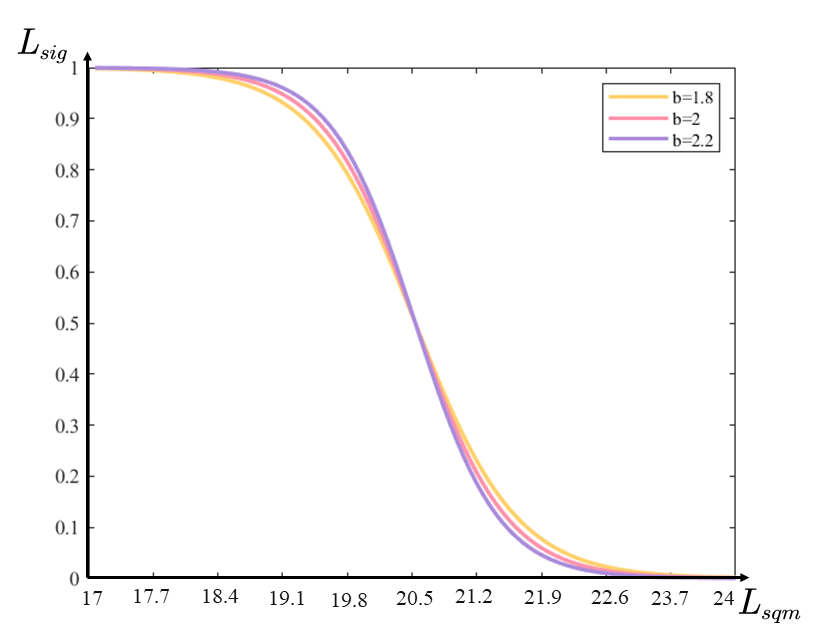
\includegraphics[width=0.5\textwidth]{sen1.png}\label{P-t gragh when rushing}
  %  \end{minipage}
%}
%\subfigure[The sensitivity of LPR]
%{
 %	\begin{minipage}[b]{0.5\linewidth}
  %      \centering
   %     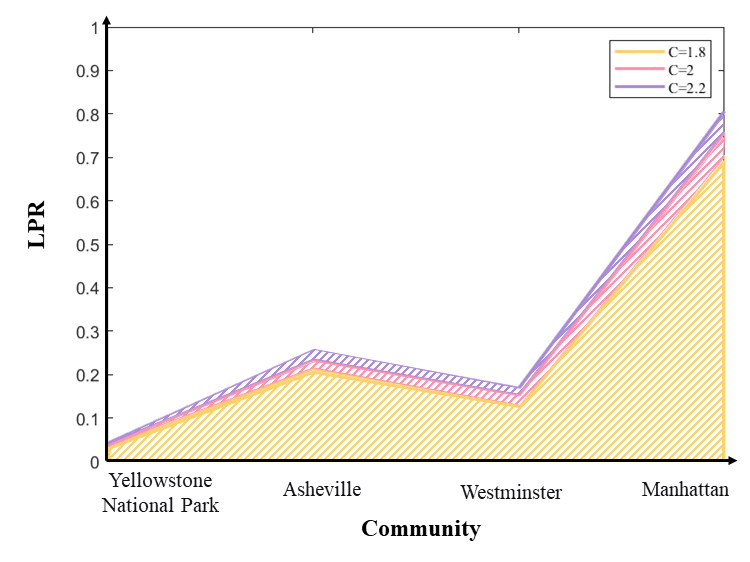
\includegraphics[width=0.5\textwidth]{sen2.png}\label{E-t graph when rushing}
    %\end{minipage}
%}
%\caption{The sensitivity of }\label{Figures when Rushing}
%\end{figure}






















The graphs show that $L_\text{sig}$ and LPR do not change much, so our model is insensitive to these two parameters and has good stability.
\section{Model Evaluation and Further Discussion}

\subsection{Strengths}
Our model offers the following strengths: 
\begin{itemize}
	\item The main strength is its enormous extensible and including all factors into a single, robust 
framework. The general applicability of our model to different communities has been shown in the previous section, and our model can also be used to assess the environmental risks caused by other pollutants.
	\item A comprehensive evaluation model for light pollution risk is scientifically sound. We combined the method of mechanism analysis and comprehensive evaluation method to obtain a more objective evaluation model.
	\item We have done good visualization work, such as framework diagrams of our work, schematic diagrams of mechanism analysis, zoning diagrams of lighting requirements, etc.Boring data may be able to reflect the law, but not as intuitive as so many images;
        \item Our model effectively achieves all the objectives, can handle large amounts of data and has the flexibility and robustness we expect.
\end{itemize}
\subsection{Weaknesses and Further Improvements}
Our model has the following limitations and related improvements: 
\begin{itemize}
	\item There are limits to the data we can collect. If we had more types and amounts of data and combined different methods of measuring light pollution, we could get a more accurate level of light pollution risk.
	\item In our hypothesis, we assumed that the variability of data within communities is negligible, but in fact, some communities have large intra-community variability, and taking this into account, we can construct more precise and detailed models to evaluate light pollution risk levels.
\end{itemize}
%Different methods may show different ranks of effect according to the users' demand, the conditions
%outside the bathtub and of the bathtub, and so on. However, according to our research in Section
%\ref{condition}, these recommended methods are still useful under various conditions, if the details
%(e.g. the temperature and the time of period) are properly adjusted. So the users can choose and
%adjust the bath strategy based on the rules below:

%\paragraph{Rule I}
%\emph{High temperature and large flux can make the water attach the optimum temperature earlier,
%	meanwhile it may cause uneven temperature and waste of water.}
%\paragraph{Rule II}
%\emph{Evenness comes from continuous inflow with appropriate temperature, a little higher than the
%	optimum temperature in usual.}
%\paragraph{Rule III}
%\emph{The best strategy to have an excellent bath is to heat %up the water before it cool down.}


\section{Pseudo-code template}
\begin{algorithm}[H]
\caption{Multivariate Linear Regression} % No number in caption
\KwData{Factor matrix (the 5 factors) $X$, Target vector $MMTTV$ at the end of each set}
\KwResult{Coefficients of the 5 factors $\beta$, Predictions $MM\hat{T}TV$}
\SetKwInOut{Input}{Input}
\SetKwInOut{Output}{Output}

\SetKwFunction{FMain}{Main}
\SetKwProg{Fn}{Function}{:}{}
\Fn{\FMain}{
  Initialize coefficients $\beta$ for each feature in $X$ to 0\;
  Set learning rate $\alpha$ and convergence threshold $\epsilon$\;
  
  \While{not converged}{
    Calculate the predicted probabilities $MM\hat{T}TV = \frac{1}{1 + e^{-X\beta}}$\;
    Calculate the gradient $k = X^T (MM\hat{T}TV - MMTTV)$\;
    Update coefficients $\beta = \beta - \alpha k$\;
    \If{$||k|| < \epsilon$}{
      set converged to True\;
    }
  }
  \KwRet{$\beta$, $MM\hat{T}TV$}
}
\end{algorithm}

\cite{kkk}

\section{Flyer}






\clearpage
123    
\clearpage
\rhead{Page 25 of 25}
\begin{thebibliography}{99}
	\addcontentsline{toc}{section}{References}  %引用部分标题（"Refenrence"）的重命名
	
	\bibitem{kkk}Green, R.F., Luginbuhl, C.B., Wainscoat, R.J. et al. The growing threat of light pollution to ground-based observatories. Astron Astrophys Rev 30, 1 (2022). 
	\bibitem{2}Léa Mariton, Christian Kerbiriou, Yves Bas, Brigitte Zanda, Isabelle Le Viol,Even low light pollution levels affect the spatial distribution and timing of activity of a “light tolerant” bat species,Environmental Pollution,Volume 305,2022,119267,ISSN 0269-7491
	\bibitem{3}Hao Q L, Ren Z F, Liu G, Wang L X, Yu J, Yu Z J. Bird risk assessment in urban ecological patch under light pollution and noise pollution stress. Acta Ecologica Sinica, 2022, 42(6): 2186-2201.
 
 
 
 \bibitem{4}LE TALLEC Thomas (May 2, 2019), What is the ecological impact of light pollution?, Encyclopedia of the Environment, Accessed February 20, 2023


\bibitem{5}S Ying, M Tang, XY Zhang. Sunlight Pollution Analysis of Glass Curtain Wall in 3D city, Geomatics and Information Science of Wuhan University. 2021,46(5):610-619. DOI:10.13203/j.whugis20200492.

\bibitem{6}Fabio Falchi,Pierantonio Cinzano,Dan Duriscoe.et al.,The new world atlas of artificial night sky brightness,Journal Article,2016, Science Advances,e1600377,2,6,10.1126/sciadv.1600377 [doi]

\bibitem{7}Daniela Grimaldi, Kathryn Reid, Ivy Mason, Chloe Warlick, Roneil Malkani, Sabra Abbott, Phyllis Zee, 012 Overnight light exposure acutely increases heart rate during sleep and decreases insulin sensitivity the following day, Sleep, Volume 44, Issue Supplement\_2, May 2021, Page A6, https://doi.org/10.1093/sleep/zsab072.011

\bibitem{8}Hölker Franz, Bolliger Janine, Davies Thomas W., Giavi Simone, Jechow Andreas, Kalinkat Gregor, Longcore Travis, Spoelstra Kamiel, Tidau Svenja, Visser Marcel E., Knop Eva.11 Pressing Research Questions on How Light Pollution Affects Biodiversity .Frontiers in Ecology and Evolution

\bibitem{9}Guanglei W, Ngarambe J, Kim G. A Comparative Study on Current Outdoor Lighting Policies in China and Korea: A Step toward a Sustainable Nighttime Environment. Sustainability. 2019; 11(14):3989. https://doi.org/10.3390/su11143989

\bibitem{10}Noam Levin, Qingling Zhang,A global analysis of factors controlling VIIRS nighttime light levels from densely populated areas,Remote Sensing of Environment,Volume 190,2017,Pages 366-382,ISSN 0034-4257,https://doi.org/10.1016/j.rse.2017.01.006.
\bibitem{11}Yang Ye, Xingyu Xue, Lingyan Huang, Muye Gan, Cheng Tong, Ke Wang, Jinsong Deng,A new perspective to map the supply and demand of artificial night light based on Loujia1-01 and urban big data,Journal of Cleaner Production,Volume 276,2020,123244,ISSN 0959-6526,https://doi.org/10.1016/j.jclepro.2020.123244.
\bibitem{12}https://www.darksky.org
\end{thebibliography}
\clearpage

\begin{center}
\underline{\Large\textbf{Report on Use of AI}}  % Centered and underlined title
\end{center}

\setlength{\parindent}{0pt}

1.OpenAI \textit{Chatgpt}

Query:123

Output:124
\\

2.OpenAI \textit{Chatgpt}

Query:123

Output:124
\\
3.OpenAI \textit{Chatgpt}

Query:123

Output:124

\end{document}
